\chapter{Fundamentação Teórica}
\label{cap:fundamentacao-teorica}

A fundamentação teórica constitui a base conceitual necessária para compreensão dos temas abordados nesta pesquisa. Nesse contexto, este 
capítulo apresenta os principais conceitos relacionados à arquitetura de software, modularidade e qualidade estrutural de sistemas orientados
a objetos. Também são discutidos os estilos arquiteturais analisados neste trabalho, bem como as métricas estruturais utilizadas para avaliar 
quantitativamente atributos relacionados ao acoplamento, à coesão e à complexidade dos sistemas estudados.

\section{Arquitetura de Software}
\label{sec:arquitetura-de-software}

A arquitetura de software está relacionada à forma como um sistema é estruturado e compreendido em um nível mais alto de abstração. 
Segundo \citeonline{bass2012}, a arquitetura de um sistema corresponde ao conjunto de estruturas necessárias para raciocinar sobre ele, 
incluindo seus elementos de software, as relações estabelecidas entre esses elementos e as propriedades associadas a ambos.

Essa definição evidencia que a arquitetura não é composta por uma única estrutura, mas por diferentes estruturas que permitem analisar 
o sistema sob perspectivas distintas. De acordo com \citeonline{bass2012}, uma estrutura pode ser compreendida como um conjunto de 
elementos ligados por algum tipo de relação. Assim, a arquitetura permite observar como os elementos do sistema se organizam e como 
se relacionam, omitindo detalhes internos que não são relevantes para a compreensão da estrutura geral.

De forma complementar, \citeonline{fowler2003} destaca que o termo arquitetura não possui uma definição única amplamente aceita, 
mas geralmente envolve dois aspectos recorrentes: a decomposição do sistema em partes de alto nível e as decisões consideradas 
difíceis de modificar posteriormente. Nesse sentido, a arquitetura representa não apenas a organização estrutural do software, 
mas também um conjunto de decisões que influenciam a forma como o sistema pode ser compreendido, mantido e evoluído.

Em determinados contextos, os elementos arquiteturais são organizados de maneiras recorrentes para solucionar problemas comuns de projeto. 
Essas composições, descritas na literatura como padrões arquiteturais, fornecem estratégias reutilizáveis para estruturar 
sistemas de software \cite{bass2012,fowler2003}. Entre os estilos relevantes para esta pesquisa destacam-se a arquitetura em camadas
e a arquitetura hexagonal, que serão discutidas nas subseções seguintes.

\subsection{Arquitetura em Camadas}
\label{sec:arquitetura-em-camadas}

A arquitetura em camadas é um padrão arquitetural no qual os elementos do sistema são organizados em níveis de responsabilidade, 
chamados camadas. Segundo \citeonline{bass2012}, esse padrão emerge quando a relação de uso entre os elementos de software ocorre 
de forma unidirecional, de modo que uma camada utiliza os serviços fornecidos pelas camadas inferiores.

De acordo com \citeonline{bass2012}, uma camada corresponde a um conjunto coerente de funcionalidades relacionadas. Em uma estrutura 
estritamente em camadas, cada camada deve utilizar apenas os serviços oferecidos pela camada imediatamente inferior. Essa organização 
estabelece uma ordem clara de dependência entre as partes do sistema, favorecendo a separação de responsabilidades e a definição de
interfaces públicas entre os níveis da aplicação.

O padrão em camadas tem como objetivo permitir que diferentes partes do sistema sejam desenvolvidas e evoluídas com menor interação
direta entre si. Para isso, o software é segmentado em unidades que agrupam módulos responsáveis por oferecer um conjunto coeso
de serviços. A Figura \ref{fig:arquitetura-camadas} apresenta uma representação simplificada desse padrão, na qual a camada superior pode utilizar
os serviços da camada imediatamente inferior, mantendo uma relação de dependência orientada de cima para baixo.

\begin{figure}[htb]
\centering
\caption{Representação do padrão arquitetural em camadas}
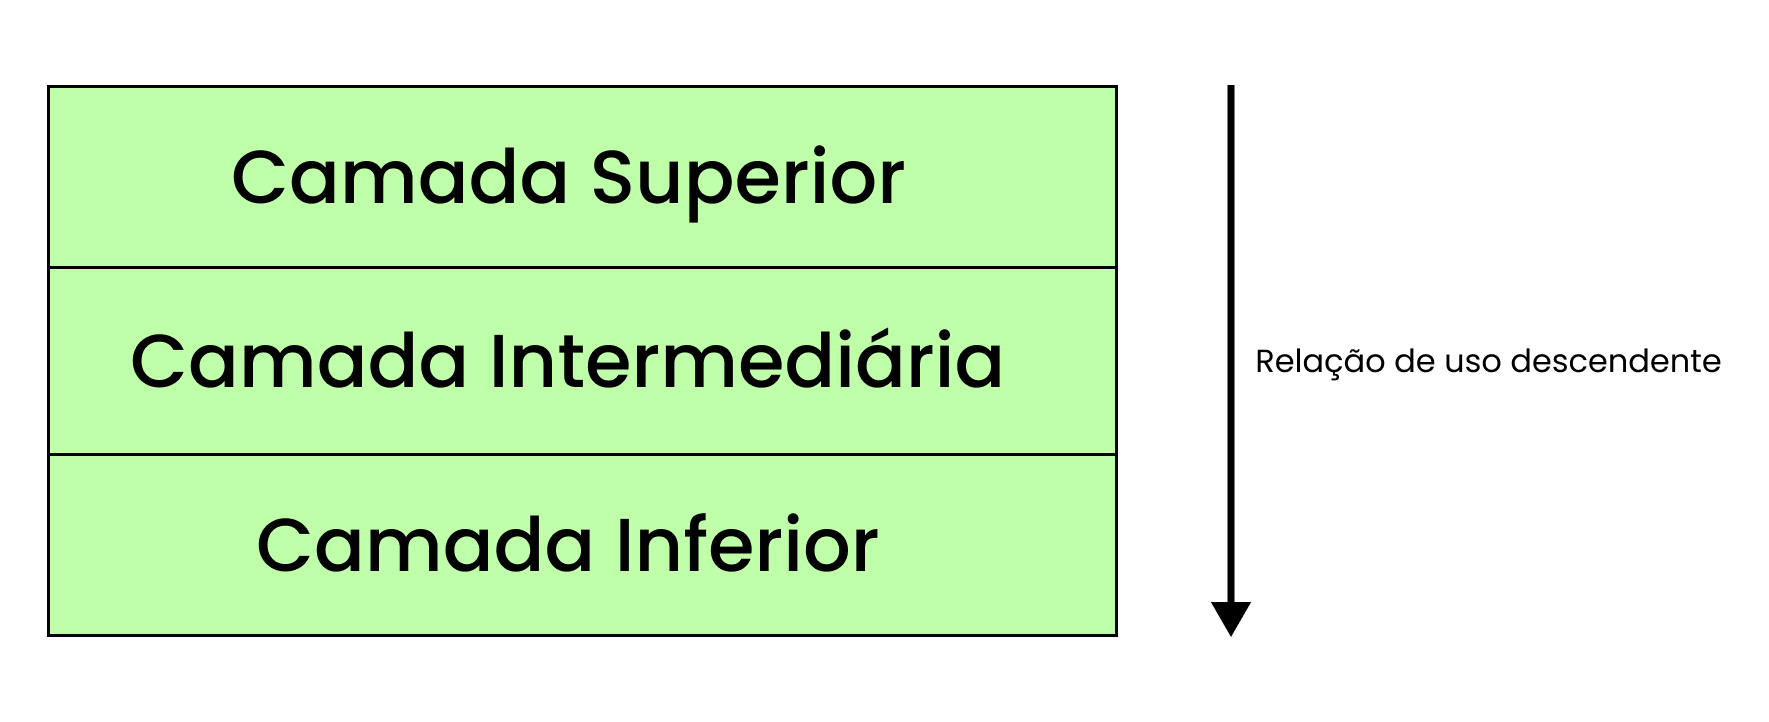
\includegraphics[width=0.65\textwidth]{figuras/arquitetura-em-camadas.png}
\label{fig:arquitetura-camadas}

\vspace{0.1cm}
\footnotesize Fonte: Elaborado pelo autor (2026), com base em \citeonline{bass2012}.

\end{figure}

Na prática, existem variações desse padrão. Embora a estrutura estrita permita apenas o uso da camada imediatamente inferior,
\citeonline{bass2012} observa que alguns sistemas permitem o acesso a camadas inferiores não adjacentes, situação conhecida
como \textit{layer bridging}. Entretanto, a ocorrência frequente desse tipo de acesso pode comprometer benefícios associados
ao padrão, como modificabilidade e portabilidade, pois aumenta o acoplamento entre partes que deveriam permanecer separadas.

Embora a arquitetura em camadas seja definida principalmente pela separação de responsabilidades e pela relação de uso entre 
camadas, sua implementação pode empregar mecanismos de abstração para reduzir dependências diretas entre seus elementos. 
Conforme discutido por \citeonline{bass2012}, as camadas expõem seus serviços por meio de interfaces públicas, permitindo que 
uma camada utilize funcionalidades fornecidas por outra sem depender de seus detalhes internos de implementação. Assim, o uso 
de interfaces entre camadas não descaracteriza a arquitetura em camadas, mas representa uma forma de controlar o acoplamento 
entre seus elementos.

Dessa forma, a arquitetura em camadas organiza o software por meio de níveis de responsabilidade e relações de dependência controladas.
Essa característica torna o padrão relevante para estudos sobre modularidade, uma vez que a forma como as camadas são estruturadas
influencia diretamente o acoplamento entre os componentes e a separação de responsabilidades no sistema.

\subsection{Arquitetura Hexagonal}
\label{sec:arquitetura-hexagonal}

A arquitetura hexagonal, também conhecida como \textit{Ports and Adapters}, foi proposta por \citeonline{cockburn2005} com 
o objetivo de permitir que uma aplicação seja desenvolvida e testada de forma isolada em relação às tecnologias externas 
utilizadas em sua execução. Nesse modelo, a aplicação deve ser capaz de interagir com diferentes mecanismos externos, como 
interfaces de usuário, bancos de dados, testes automatizados, scripts ou outros sistemas, sem que suas regras internas dependam
diretamente dessas tecnologias \cite{cockburn2005}.

Segundo \citeonline{cockburn2005}, a motivação central desse padrão está relacionada à necessidade de evitar o acoplamento entre a 
lógica da aplicação e os elementos externos ao sistema. O autor destaca que problemas semelhantes ocorrem tanto quando regras de negócio 
são incorporadas à interface com o usuário quanto quando a lógica da aplicação passa a depender diretamente de bancos de dados ou serviços 
externos. Nesses casos, alterações tecnológicas podem afetar partes centrais do sistema, dificultando testes e a substituição de mecanismos 
externos.

A solução proposta pela arquitetura hexagonal consiste em estabelecer uma separação entre o interior e o exterior da aplicação. O núcleo 
da aplicação comunica-se com elementos externos por meio de portas, que representam interfaces ou protocolos de interação. Os adaptadores, 
por sua vez, são responsáveis por converter chamadas, mensagens ou sinais específicos de uma tecnologia externa para uma forma compreensível 
pela aplicação, e vice-versa \cite{cockburn2005}. A Figura \ref{fig:arquitetura-hexagonal} apresenta uma representação desse padrão.

\begin{figure}[htb]
\centering
\caption{Representação do padrão arquitetural hexagonal}
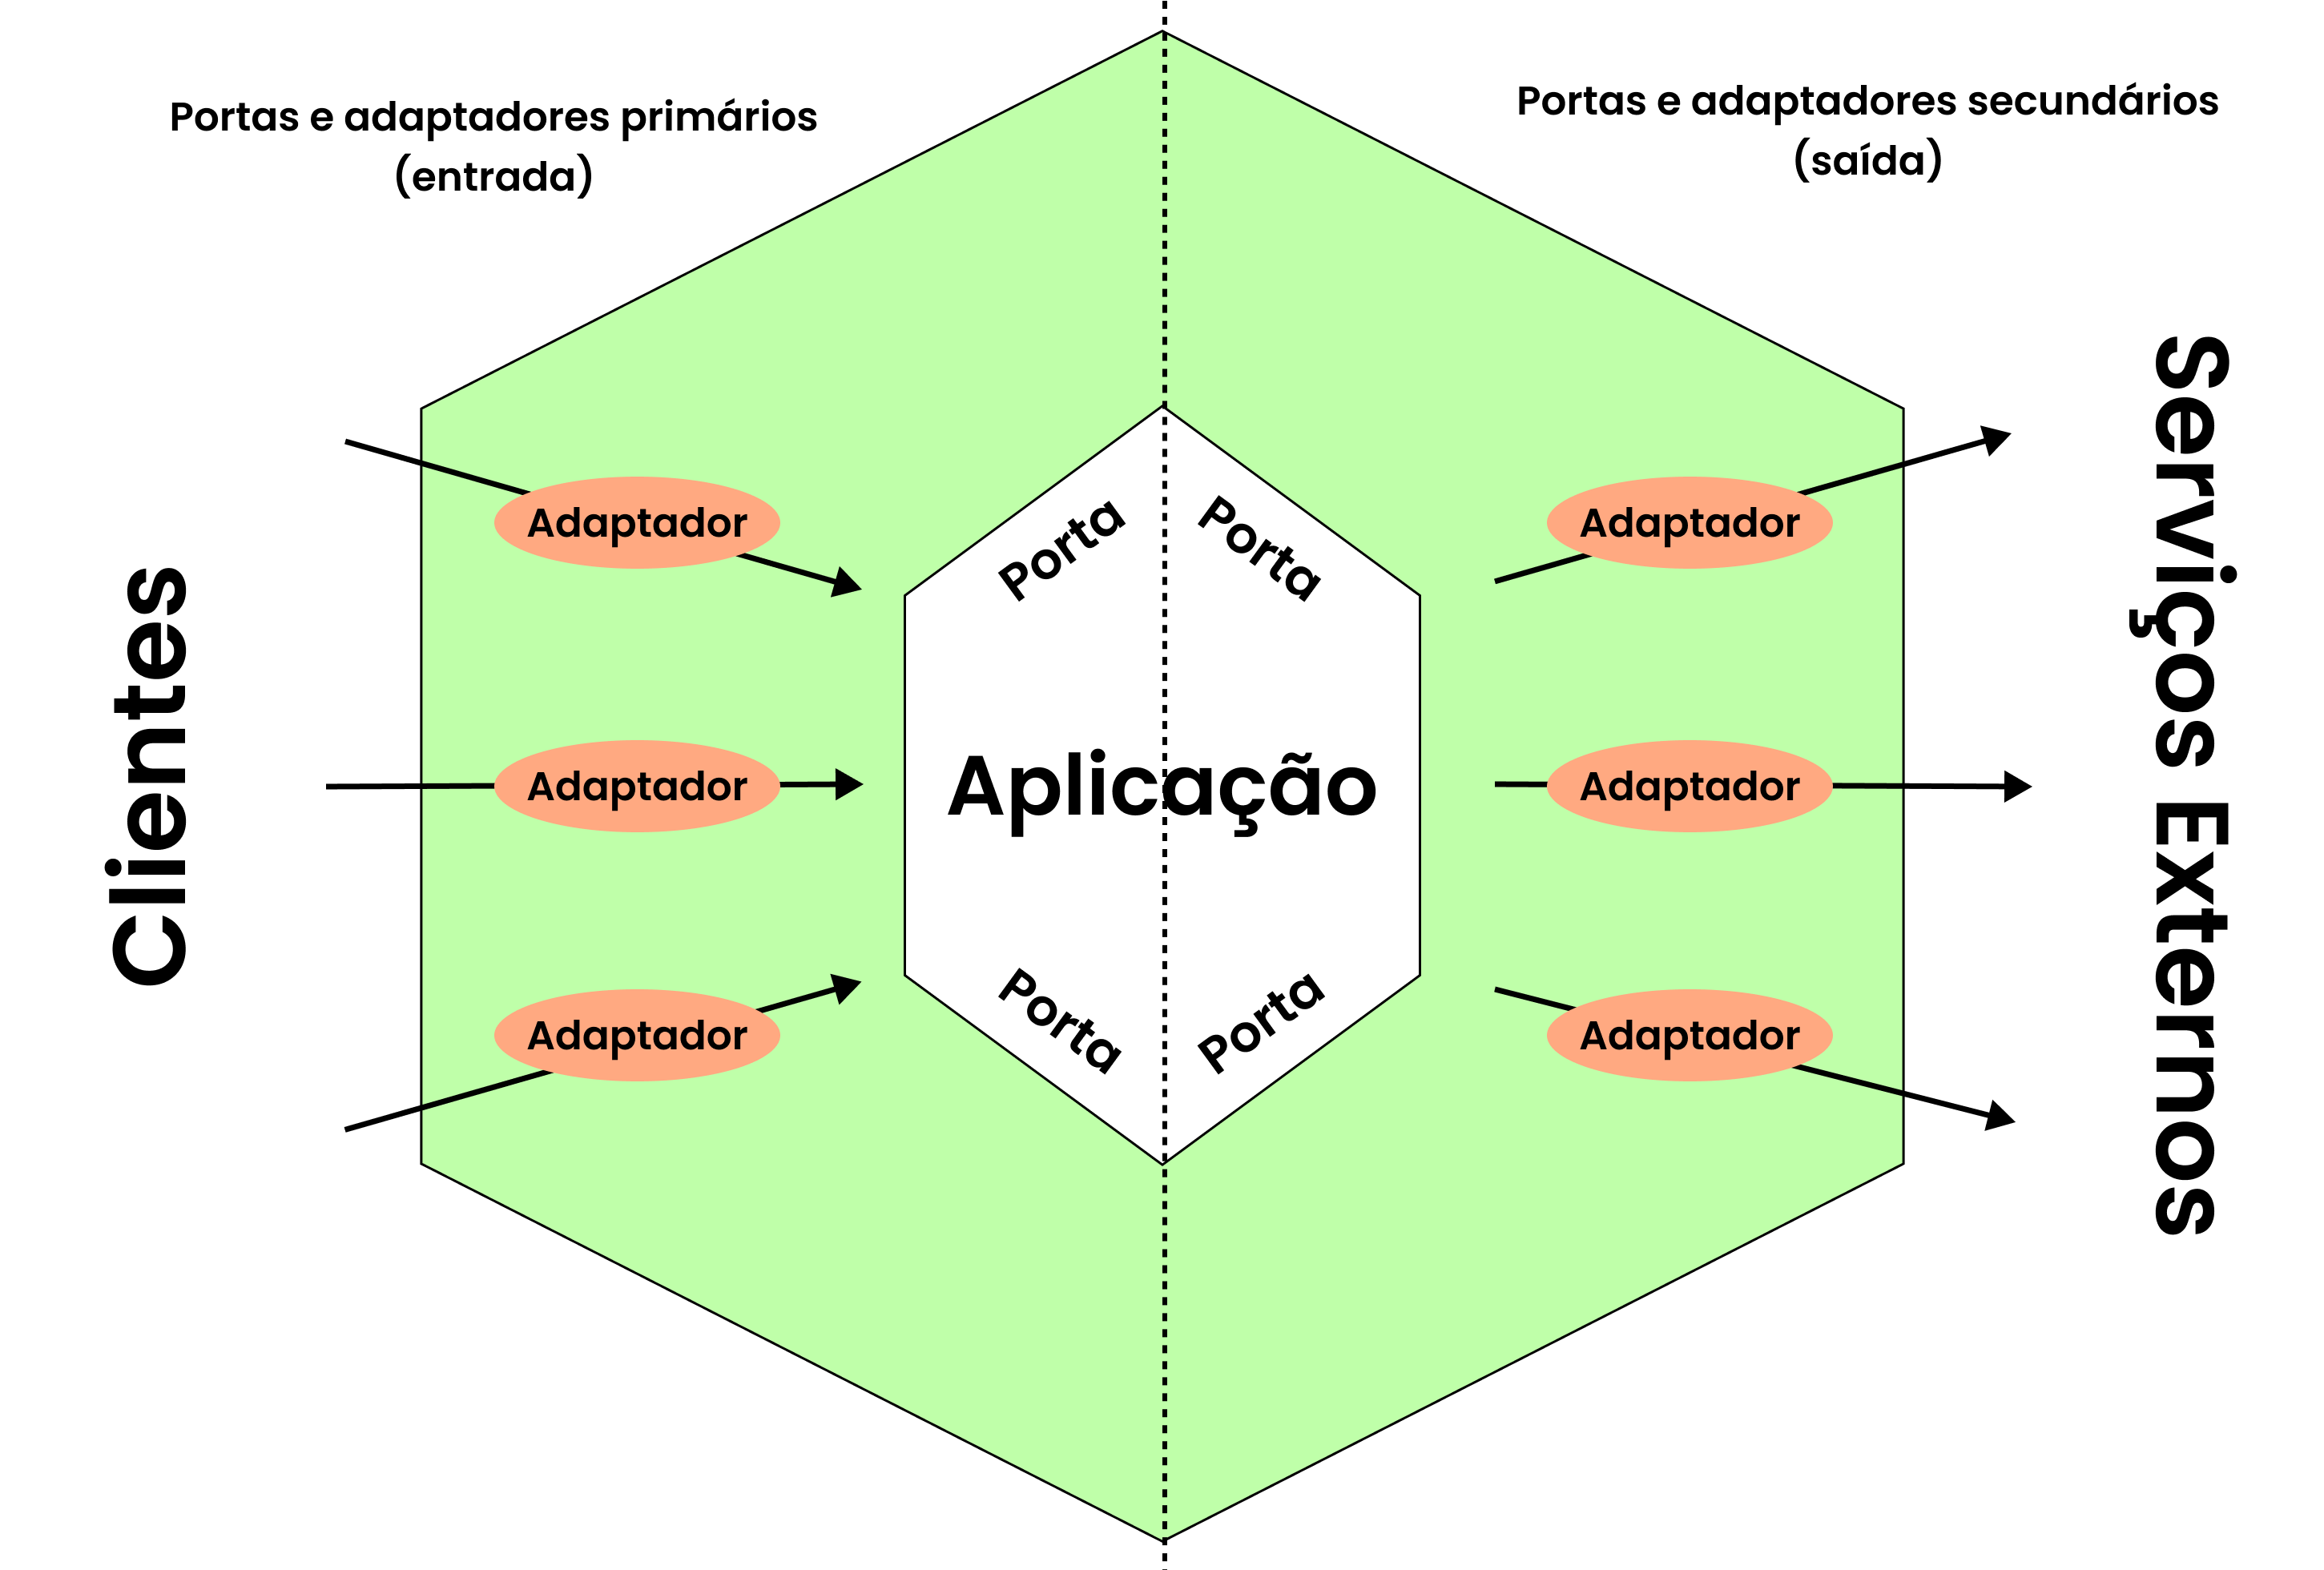
\includegraphics[width=0.90\textwidth]{figuras/arquitetura-hexagonal.png}
\label{fig:arquitetura-hexagonal}

\vspace{0.1cm}
\footnotesize Fonte: Elaborado pelo autor (2026), com base em \citeonline{cockburn2005}.

\end{figure}

Nesse padrão, o termo ``hexagonal'' não indica que a aplicação deve possuir exatamente seis lados ou seis interfaces. De acordo 
com \citeonline{cockburn2005}, o uso do hexágono busca representar visualmente a existência de múltiplas portas ao redor da aplicação, 
destacando a separação entre o núcleo interno e os elementos externos. Assim, diferentes tipos de adaptadores podem ser conectados às 
portas da aplicação, permitindo substituir uma interface gráfica por testes automatizados ou trocar um banco de dados real por uma 
implementação em memória, sem alterar as regras internas do sistema \cite{cockburn2005}.

Em implementações orientadas a objetos, as portas podem ser representadas por interfaces de programação que definem os serviços oferecidos 
ou requeridos pelo núcleo da aplicação. Os adaptadores implementam essas portas e conectam a aplicação a tecnologias específicas, como 
interfaces gráficas, APIs, mecanismos de persistência ou serviços externos \cite{cockburn2005}. Essa organização favorece a independência 
tecnológica, pois as regras internas da aplicação permanecem separadas dos detalhes de infraestrutura e integração.

A arquitetura hexagonal diferencia-se da arquitetura em camadas por enfatizar a relação entre o interior e o exterior da aplicação, em vez 
de representar o sistema apenas como uma sequência vertical de camadas \cite{cockburn2005}. Enquanto a arquitetura em camadas organiza o 
software em níveis hierárquicos de responsabilidade, a arquitetura hexagonal concentra-se na proteção do núcleo da aplicação contra 
dependências tecnológicas externas. Essa característica torna o padrão relevante para estudos sobre modularidade, uma vez que a forma 
como portas e adaptadores são definidos pode influenciar as dependências entre componentes e a separação entre regras de negócio e 
infraestrutura.

\section{Modularidade em Software}
\label{sec:modularidade-em-software}

A modularidade está diretamente relacionada à forma como um sistema é dividido em partes menores e mais gerenciáveis \cite{parnas1972}. 
Em sistemas modulares, as funcionalidades são organizadas em unidades relativamente independentes, permitindo que cada módulo 
desempenhe responsabilidades específicas e possa ser compreendido, desenvolvido e modificado com menor impacto sobre os demais 
componentes do sistema.

Um dos trabalhos pioneiros sobre modularização foi apresentado por \citeonline{parnas1972}, que argumenta que a decomposição de sistemas
em módulos deve ser realizada de forma a minimizar a propagação de mudanças entre diferentes partes do software. Segundo o autor, uma 
estrutura modular adequada reduz a complexidade do desenvolvimento e facilita atividades de manutenção, evolução e correção de defeitos.

De acordo com \citeonline{sommerville2011}, sistemas complexos podem ser organizados em componentes com responsabilidades específicas, 
favorecendo sua compreensão e reduzindo a complexidade do desenvolvimento. Essa decomposição também contribui para a reutilização de 
funcionalidades, uma vez que componentes bem definidos podem ser empregados em diferentes contextos com menor necessidade de modificações.

A importância da modularidade está associada à capacidade de controlar a complexidade inerente ao desenvolvimento de software. Segundo
\citeonline{pressman2010}, sistemas de grande porte tornam-se progressivamente mais difíceis de compreender e modificar quando
apresentam dependências excessivas entre seus componentes. Nesse contexto, a modularização surge como uma estratégia para organizar 
responsabilidades e limitar o impacto das mudanças realizadas ao longo do ciclo de vida do software.

Embora o conceito de modularidade seja amplamente discutido na literatura, sua avaliação objetiva não é uma tarefa trivial. Conforme discutido por
\citeonline{fenton2015}, atributos relacionados à qualidade interna do software frequentemente apresentam natureza abstrata e, por esse motivo,
podem ser avaliados por meio de indicadores quantitativos. Dessa forma, características associadas à modularidade são frequentemente 
investigadas por intermédio de métricas estruturais capazes de mensurar propriedades observáveis do código-fonte.

Entre os atributos frequentemente associados à avaliação da modularidade e da qualidade estrutural de sistemas orientados a objetos 
destacam-se o acoplamento, a coesão e a complexidade estrutural \cite{pressman2010,fenton2015}. Assim, esses atributos serão discutidos
nas subseções seguintes pois permitem analisar diferentes aspectos da organização estrutural do software.

\subsection{Acoplamento}
\label{sec:acoplamento}

O acoplamento representa o grau de dependência existente entre módulos, componentes ou classes de um sistema de software. 
Em sistemas orientados a objetos, essa dependência ocorre quando uma classe estabelece relacionamentos com outras classes para 
utilizar seus serviços, trocar dados ou acessar elementos necessários à implementação de suas responsabilidades \cite{pressman2010}.

Segundo \citeonline{pressman2010}, à medida que componentes se tornam mais interdependentes, o grau de acoplamento aumenta. 
Como consequência, alterações realizadas em um componente tendem a produzir impactos em outros componentes relacionados.

Embora algum nível de acoplamento seja inevitável em sistemas de software, uma vez que seus componentes precisam se comunicar 
para executar suas funcionalidades, \citeonline{pressman2010} destaca que o projeto deve buscar reduzi-lo sempre que possível. 
Sistemas com baixo acoplamento favorecem a independência entre módulos, limitam a propagação de mudanças e facilitam a reutilização
dos componentes.

O conceito de baixo acoplamento também está relacionado ao princípio da ocultação de informações (\textit{information hiding}) proposto 
por \citeonline{parnas1972}. Segundo esse princípio, os módulos devem expor apenas as informações estritamente necessárias para sua 
utilização, preservando seus detalhes internos de implementação. Dessa forma, modificações realizadas em um componente tendem a produzir 
menor impacto sobre os demais elementos do sistema.

O acoplamento constitui, portanto, um atributo importante para a organização de sistemas modulares, uma vez que influencia a independência
entre componentes e a propagação de mudanças ao longo do software. Entretanto, a qualidade estrutural de um sistema não depende apenas
das relações estabelecidas entre seus módulos, mas também da organização interna de cada um deles. Esse aspecto é representado pelo 
conceito de coesão, discutido na subseção seguinte.

\subsection{Coesão}
\label{sec:coesao}

A coesão refere-se ao grau de relacionamento existente entre os elementos internos de um módulo ou classe. Em sistemas orientados a
objetos, um componente é considerado coeso quando encapsula atributos e operações fortemente relacionados entre si e direcionados
a um mesmo propósito \cite{pressman2010}.

Segundo \citeonline{pressman2010}, a coesão constitui uma característica desejável em projetos de software, pois componentes cujos 
elementos estão fortemente relacionados tendem a ser mais simples de implementar, testar e manter. Em contrapartida, componentes que
agrupam funcionalidades pouco relacionadas costumam apresentar maior complexidade e dificultam atividades de manutenção e evolução do
sistema.

De acordo com \citeonline{bass2012}, a coesão está diretamente relacionada ao grau de associação entre as responsabilidades atribuídas 
a um módulo. Os autores descrevem esse atributo como uma medida da ``unidade de propósito'' (\textit{unity of purpose}) de um componente, 
indicando que módulos altamente coesos tendem a concentrar responsabilidades relacionadas, reduzindo a probabilidade de que uma mudança 
em uma responsabilidade afete funcionalidades distintas.

Assim como o acoplamento descreve as dependências existentes entre diferentes componentes, a coesão concentra-se na organização interna 
de cada módulo. Dessa forma, sistemas modulares buscam simultaneamente reduzir as dependências entre componentes e concentrar responsabilidades
relacionadas em unidades bem definidas.

Nesse contexto, a coesão constitui um atributo relevante para avaliação da modularidade de sistemas de software, complementando a análise do acoplamento 
ao considerar a forma como responsabilidades e funcionalidades são organizadas no interior de cada componente. Além disso, a avaliação da qualidade estrutural 
também envolve a análise da complexidade resultante da organização e das relações estabelecidas entre os elementos do sistema.

\subsection{Complexidade}
\label{sec:complexidade}

Neste trabalho, a complexidade é compreendida sob uma perspectiva estrutural, estando relacionada à dificuldade de compreender a organização de 
um sistema de software e as relações estabelecidas entre seus elementos \cite{pressman2010,fenton2015}. Em sistemas orientados a objetos, essa 
complexidade pode ser observada a partir da forma como classes, métodos e dependências se organizam e interagem ao longo da estrutura do sistema.

Segundo \citeonline{pressman2010}, existem diferentes formas de compreender a complexidade de software. No contexto de projetos orientados a objetos, 
a complexidade pode ser analisada a partir de características estruturais, especialmente pela forma como as classes se relacionam entre si. Dessa maneira, 
sistemas com maior quantidade de elementos interdependentes tendem a exigir maior esforço de compreensão, manutenção e evolução.

De forma complementar, \citeonline{fenton2015} associa a complexidade estrutural à complexidade das conexões entre os elementos de um modelo de sistema. 
Para os autores, essa complexidade depende do número de ligações existentes entre os elementos, indicando que sistemas com maior quantidade de relações 
estruturais tendem a apresentar maior complexidade interna. Assim, a análise da complexidade estrutural permite observar não apenas a quantidade de elementos 
presentes no sistema, mas também como esses elementos estão conectados.

No contexto desta pesquisa, a complexidade é analisada a partir de propriedades observáveis no código-fonte dos sistemas. Dessa forma, não se pretende
avaliar a complexidade algorítmica ou o desempenho das aplicações, mas sim características relacionadas à organização das classes, à quantidade de operações
e ao potencial de interação entre os componentes.

Assim, a complexidade estrutural complementa os conceitos de acoplamento e coesão na avaliação da qualidade estrutural do software. Enquanto o acoplamento 
considera as dependências entre classes e a coesão considera a organização interna de cada módulo, a complexidade contribui para compreender o esforço necessário 
para analisar, modificar e evoluir os elementos estruturais do sistema.

\section{Métricas de Software}
\label{sec:metricas-de-software}

A mensuração é uma atividade importante para analisar características de sistemas de software de forma objetiva. 
Segundo \citeonline{fenton2015}, medição é o processo pelo qual números ou símbolos são atribuídos a atributos de 
entidades do mundo real, de acordo com regras claramente definidas. Dessa forma, o processo de medição não avalia uma 
entidade de maneira genérica, mas atributos específicos que se deseja observar.

No contexto da Engenharia de Software, métricas permitem representar quantitativamente características de sistemas, componentes 
ou processos. De acordo com \citeonline{sommerville2011}, uma métrica de software corresponde a uma característica de um sistema 
de software, de sua documentação ou de seu processo de desenvolvimento que pode ser medida objetivamente. Entre essas características, 
podem ser observados aspectos relacionados ao tamanho, à complexidade, à ocorrência de falhas ou ao esforço necessário para 
desenvolver componentes.

As medições de um sistema de software podem ser utilizadas para apoiar a análise de atributos de qualidade. Segundo 
\citeonline{sommerville2011}, características de componentes podem ser medidas e utilizadas para avaliar atributos mais gerais 
do sistema. Nesta pesquisa, esse princípio é aplicado à análise de características estruturais de classes, como dependências, coesão 
e complexidade, permitindo observar diferenças na organização interna dos sistemas estudados.

Embora forneçam valores objetivos sobre características observáveis do software, métricas não devem ser interpretadas isoladamente 
como medidas absolutas de qualidade. \citeonline{fenton2015} destacam que toda ação de medição deve estar associada a um objetivo 
ou necessidade claramente definida. Assim, os valores obtidos por métricas precisam ser analisados de acordo com o contexto do 
sistema e com o propósito da avaliação.

No contexto deste trabalho, as métricas de software são utilizadas como indicadores quantitativos para apoiar a análise da modularidade 
e da qualidade estrutural dos sistemas estudados. Como o foco está em sistemas orientados a objetos, interessam especialmente métricas 
extraídas do código-fonte, capazes de fornecer indicadores sobre características estruturais relacionadas a classes, dependências, coesão 
e complexidade. Essas métricas são discutidas na seção seguinte.

\section{Métricas Estruturais em Sistemas Orientados a Objetos}
\label{sec:metricas-estruturais-em-sistemas-orientados-a-objetos}

Em sistemas orientados a objetos, a estrutura do software é organizada principalmente a partir de classes, objetos, métodos, interfaces 
e relações entre esses elementos. \citeonline{fenton2015} destacam que projetos e implementações orientados a objetos são construídos 
com base em classes, que definem conjuntos de objetos instanciáveis e agrupam métodos relacionados ao comportamento desses objetos. 
Além disso, linguagens orientadas a objetos podem incluir mecanismos como interfaces, herança e ligação dinâmica, que aumentam a 
expressividade dos desenvolvedores, mas também podem tornar projetos e implementações mais complexos.

Essa forma de organização torna necessária a utilização de métricas capazes de representar características próprias do paradigma 
orientado a objetos. \citeonline{chidamber1994} argumentam que métricas desenvolvidas para abordagens tradicionais de desenvolvimento 
não se ajustam diretamente a conceitos como classes, herança, encapsulamento e troca de mensagens. Por esse motivo, os autores 
propõem um conjunto de métricas voltado especificamente à avaliação de projetos orientados a objetos.

A classe ocupa papel central nesse tipo de avaliação. De acordo com \citeonline{pressman2010}, a classe é uma unidade fundamental 
em sistemas orientados a objetos, pois encapsula dados e operações, pode participar de hierarquias de herança e colabora com 
outras classes para realizar as funcionalidades do sistema. Dessa forma, métricas aplicadas no nível de classe podem fornecer 
informações relevantes sobre características estruturais do software, como acoplamento, coesão, complexidade e comunicação 
entre componentes.

De forma semelhante, \citeonline{chidamber1994} afirmam que o projeto de classes é central no paradigma orientado a objetos, 
razão pela qual as métricas propostas pelos autores foram definidas para capturar aspectos estruturais relacionados às classes 
e às relações estabelecidas entre elas. Essas métricas são consideradas estáticas, pois podem ser coletadas a partir da estrutura 
do projeto ou da implementação, sem a necessidade de executar o sistema.

A suíte CK, proposta por Chidamber e Kemerer, é composta por seis métricas orientadas a classes: \textit{Weighted Methods per Class} 
(WMC), \textit{Depth of Inheritance Tree} (DIT), \textit{Number of Children} (NOC), \textit{Coupling Between Object Classes} (CBO), 
\textit{Response For a Class} (RFC) e \textit{Lack of Cohesion in Methods} (LCOM) \cite{chidamber1994}. Essas métricas abordam 
diferentes dimensões do projeto orientado a objetos, incluindo complexidade interna da classe, uso de herança, dependências 
entre classes, conjunto de respostas possíveis e coesão entre métodos.

Além das métricas da suíte CK, medidas relacionadas ao fluxo de dependências entre componentes também são utilizadas para analisar 
a estrutura de sistemas de software. Nesse contexto, Fan-In e Fan-Out são discutidas na literatura como medidas associadas, 
respectivamente, à quantidade de elementos que dependem de um componente e à quantidade de elementos dos quais um componente 
depende \cite{yourdon1978,sommerville2011}. Essas métricas complementam a análise de acoplamento ao permitir observar a direção 
e a concentração das dependências no sistema.

No contexto desta pesquisa, o interesse recai sobre métricas relacionadas à modularidade e à qualidade estrutural dos sistemas 
estudados. Por esse motivo, são consideradas métricas associadas principalmente ao acoplamento, à coesão e à complexidade 
estrutural das classes. As subseções seguintes apresentam as métricas utilizadas no estudo, incluindo CBO, LCOM, RFC, WMC, 
Fan-In e Fan-Out, discutindo sua relação com os atributos estruturais analisados.

É importante destacar que algumas métricas orientadas a objetos podem apresentar variações de definição e implementação na 
literatura e em ferramentas de análise estática. A própria definição da WMC, por exemplo, considera a soma das complexidades 
dos métodos de uma classe, mas \citeonline{chidamber1994} indicam que a forma específica de medir essa complexidade pode 
depender da implementação adotada. Assim, neste capítulo as métricas são apresentadas em seu significado conceitual e em 
sua relação com os atributos analisados, enquanto a forma específica de operacionalização adotada pela ferramenta utilizada 
nesta pesquisa é descrita na Metodologia.

\subsection{\textit{Coupling Between Object Classes} (CBO)}
\label{sec:cbo}

A métrica \textit{Coupling Between Object Classes} (CBO) tem como objetivo representar o grau 
de acoplamento existente entre uma classe e as demais classes do sistema. Segundo \citeonline{chidamber1994}, o CBO de uma classe 
corresponde ao número de outras classes às quais ela está acoplada. Essa relação ocorre quando métodos de uma classe utilizam métodos 
ou variáveis de instância definidos em outra classe.

Em sistemas orientados a objetos, valores elevados de CBO indicam maior dependência entre classes. De acordo com 
\citeonline{sommerville2011}, classes são consideradas acopladas quando métodos de uma classe utilizam métodos ou 
variáveis definidos em outra. Assim, quanto maior o valor de CBO, maior tende a ser a dependência da classe em relação 
a outros elementos do sistema, aumentando a possibilidade de que alterações em uma classe produzam impactos em outras partes 
do programa.

A interpretação dessa métrica também está associada à modularidade e à reutilização. \citeonline{pressman2010} observa que, 
à medida que o valor de CBO aumenta, a reutilização de uma classe tende a diminuir, pois a classe passa a depender de um número 
maior de colaborações externas. Além disso, altos valores de CBO podem dificultar modificações e testes, uma vez que mudanças 
em classes acopladas podem exigir maior atenção aos efeitos propagados pelo sistema.

Apesar de sua relevância, o CBO deve ser interpretado com cautela. \citeonline{fenton2015} destacam que a métrica contabiliza o 
número de classes às quais uma classe está acoplada, e não necessariamente o número total de conexões existentes entre elas. 
Dessa forma, duas classes podem apresentar o mesmo valor de CBO mesmo que possuam intensidades diferentes de interação. Assim, 
o CBO deve ser compreendido como um indicador do alcance do acoplamento de uma classe, e não como uma medida completa de todas 
as dependências internas existentes no sistema.

Neste trabalho, o CBO será interpretado como um indicador do acoplamento estrutural das classes, permitindo observar quais partes
dos sistemas concentram maior número de dependências com outros elementos do código. Dessa forma, o CBO contribui para investigar 
como a arquitetura em camadas e a arquitetura hexagonal se refletem nas dependências estruturais observadas no código-fonte.

\subsection{\textit{Lack of Cohesion in Methods} (LCOM)}
\label{sec:lcom}

A métrica \textit{Lack of Cohesion in Methods} (LCOM) indica a falta de coesão interna de uma classe. 
Diferentemente de métricas que avaliam dependências entre classes, a LCOM concentra-se na relação entre os 
métodos de uma classe e os atributos ou variáveis de instância utilizados por esses métodos.

Segundo \citeonline{fenton2015}, a coesão de uma classe pode ser caracterizada pelo grau de relacionamento entre seus métodos locais 
e suas variáveis de instância. Nesse sentido, métodos que acessam ou modificam atributos em comum tendem a indicar maior proximidade 
funcional dentro da classe. Por outro lado, quando os métodos utilizam conjuntos distintos de atributos, a classe pode apresentar 
menor coesão interna.

A LCOM é considerada uma métrica inversa de coesão, pois valores mais altos indicam menor coesão entre os métodos da classe 
\cite{fenton2015}. Essa interpretação também é discutida por \citeonline{pressman2010}, ao destacar que valores elevados de 
LCOM podem indicar maior complexidade no projeto da classe. De modo geral, busca-se manter a coesão elevada, o que corresponde 
a valores mais baixos para métricas de falta de coesão.

Entretanto, a definição e a utilidade da LCOM devem ser interpretadas com cautela. \citeonline{sommerville2011} observa que essa 
métrica existe em diferentes variações e que seu valor tem sido objeto de debate na literatura. De forma semelhante, 
\citeonline{fenton2015} destacam limitações associadas à formulação original da métrica, especialmente por não ser normalizada. 
Assim, a LCOM deve ser compreendida como um indicador relacionado à coesão interna da classe, e não como uma medida absoluta da 
qualidade de seu projeto.

Nesse trabalho, a LCOM é considerada como uma métrica relacionada à coesão interna das classes. A forma específica de 
operacionalização adotada neste trabalho é apresentada na Metodologia, juntamente com as demais métricas utilizadas na análise 
estrutural dos sistemas.

\subsection{\textit{Response For a Class} (RFC)}
\label{sec:rfc}

A métrica \textit{Response For a Class} (RFC) representa o tamanho do conjunto de respostas possíveis de uma classe. De acordo com 
\citeonline{chidamber1994}, o conjunto de respostas de uma classe corresponde ao conjunto de métodos que podem ser potencialmente 
executados em resposta a uma mensagem recebida por um objeto dessa classe.

Esse conjunto inclui tanto os métodos definidos na própria classe quanto os métodos externos que podem ser invocados por seus
métodos locais. Nesse sentido, \citeonline{fenton2015} descrevem a RFC como a soma entre o número de métodos locais e o número 
de métodos externos chamados por esses métodos. Dessa forma, a métrica permite observar não apenas a quantidade de operações 
diretamente disponíveis em uma classe, mas também o potencial de interação dessa classe com outros elementos do sistema.

Valores elevados de RFC indicam que uma classe possui um conjunto maior de comportamentos potencialmente executáveis em resposta 
a uma chamada. \citeonline{pressman2010} observa que, à medida que a RFC aumenta, também tende a aumentar o esforço necessário 
para testar a classe, pois cresce o número de métodos que podem participar das sequências de execução. De forma semelhante, 
\citeonline{sommerville2011} relaciona valores mais altos de RFC a maior complexidade da classe, uma vez que mais métodos 
podem ser acionados a partir de uma mensagem recebida.

Apesar de sua utilidade, a RFC deve ser interpretada como um indicador do tamanho do conjunto de respostas de uma classe, e 
não como uma representação completa de seu comportamento em tempo de execução. Conforme discutido por \citeonline{fenton2015}, 
a métrica contabiliza os métodos presentes no conjunto de respostas, mas não necessariamente o número total de chamadas 
realizadas ou a frequência com que essas chamadas ocorrem. Assim, classes com valores semelhantes de RFC podem apresentar 
diferentes intensidades de interação interna ou externa.

No contexto desta pesquisa, a RFC é utilizada como indicador relacionado à complexidade estrutural e ao potencial de interação 
das classes. A análise dessa métrica permite observar se os estilos arquiteturais estudados estão associados a classes com 
maior ou menor conjunto de respostas possíveis, contribuindo para a comparação da organização estrutural dos sistemas analisados.

\subsection{\textit{Weighted Methods per Class} (WMC)}
\label{sec:wmc}

A métrica \textit{Weighted Methods per Class} (WMC) está relacionada à quantidade e à complexidade dos métodos definidos em uma 
classe. Segundo \citeonline{chidamber1994}, a WMC é calculada a partir da soma dos pesos atribuídos aos métodos de uma classe, 
em que cada peso representa um fator de complexidade associado ao respectivo método.

A interpretação da WMC depende da forma como os pesos dos métodos são definidos. \citeonline{fenton2015} destacam que, quando 
todos os métodos recebem peso igual a 1, a WMC passa a representar uma medida de tamanho da classe, correspondendo ao número 
de métodos nela definidos. Dessa forma, a métrica pode ser compreendida tanto como uma medida de complexidade quanto como uma 
medida de tamanho, dependendo da estratégia adotada para atribuição dos pesos.

De acordo com \citeonline{pressman2010}, o número de métodos e a complexidade desses métodos são indicadores razoáveis do 
esforço necessário para implementar e testar uma classe. O autor também observa que, à medida que o número de métodos cresce, 
a classe tende a se tornar mais específica da aplicação, o que pode limitar seu potencial de reutilização. Assim, valores 
elevados de WMC podem indicar classes com maior responsabilidade interna e maior esforço de compreensão.

Semelhantemente, \citeonline{sommerville2011} relaciona valores mais altos de WMC a classes mais complexas e potencialmente 
mais difíceis de compreender. Classes com muitos métodos ou métodos mais complexos podem concentrar diferentes responsabilidades, 
o que pode afetar sua coesão lógica e dificultar sua reutilização em hierarquias de herança ou em outros contextos do sistema.

No âmbito desta pesquisa, a WMC é utilizada como indicador relacionado à complexidade estrutural das classes. A análise dessa 
métrica permite observar se os sistemas estudados apresentam classes com maior concentração de comportamento ou maior complexidade
interna, contribuindo para a comparação entre a organização estrutural da arquitetura em camadas e da arquitetura hexagonal.

\subsection{\textit{Fan-In}}
\label{sec:fan-in}

A métrica \textit{Fan-In} está ligada à quantidade de elementos que direcionam dependências, chamadas ou fluxos para um
determinado módulo, função, método ou componente. Em termos gerais, ela representa o número de partes do sistema que utilizam 
ou dependem de um elemento analisado, permitindo observar o grau de entrada de dependências sobre esse elemento.

Segundo \citeonline{fenton2015}, o \textit{fan-in} de um módulo pode ser compreendido como a quantidade de fluxos locais que 
terminam nesse módulo, juntamente com as estruturas de dados das quais ele recupera informações. Embora essa definição esteja 
associada a uma visão modular mais geral, ela evidencia a ideia central da métrica: identificar quantos fluxos ou dependências 
chegam a uma unidade do sistema.

De forma semelhante, \citeonline{sommerville2011} define \textit{fan-in} como uma medida do número de funções ou métodos que 
chamam uma determinada função ou método. Nesse sentido, valores elevados de \textit{fan-in} indicam que o elemento analisado 
é utilizado por várias partes do sistema, podendo representar uma unidade central na estrutura do software. Entretanto, essa 
centralidade também implica maior atenção, pois alterações nesse elemento podem produzir efeitos em diferentes partes do sistema 
que dependem dele.

A interpretação do \textit{Fan-In} não deve ser feita apenas de forma negativa. \citeonline{yourdon1978} observa que, em determinados 
contextos, aumentar o \textit{fan-in} pode ser desejável, pois indica que funcionalidades comuns estão sendo reutilizadas em vez de 
duplicadas em diferentes partes do sistema. Nesse sentido, o \textit{Fan-In} pode estar associado à modularidade quando representa o 
reaproveitamento adequado de responsabilidades bem definidas.

Porém, \citeonline{yourdon1978} também ressalta que o aumento do \textit{fan-in} não deve ocorrer a qualquer custo. Agrupar 
funcionalidades não relacionadas em um único módulo apenas para aumentar seu uso pode comprometer a coesão e gerar componentes 
excessivamente genéricos ou difíceis de manter. Assim, valores elevados de \textit{Fan-In} devem ser analisados em conjunto com 
outras métricas, especialmente aquelas relacionadas à coesão e ao acoplamento.

Nesse sentido, o \textit{Fan-In} é utilizado como indicador da quantidade de dependências que chegam a uma classe. 
A análise dessa métrica permite identificar classes mais centrais ou mais reutilizadas dentro da estrutura dos sistemas estudados. 
Dessa forma, o \textit{Fan-In} contribui para compreender como as dependências se distribuem nas arquiteturas analisadas e quais 
classes concentram maior número de relações de entrada.

\subsection{\textit{Fan-Out}}
\label{sec:fan-out}

A métrica \textit{Fan-Out} relaciona-se à quantidade de dependências, chamadas ou fluxos que saem de um determinado 
módulo, função, método ou componente. Enquanto o \textit{Fan-In} observa quantos elementos utilizam uma unidade do sistema, 
o \textit{Fan-Out} considera quantos elementos são utilizados por essa unidade. Dessa forma, a métrica permite analisar o 
grau em que um elemento depende de outros para executar suas responsabilidades.

Segundo \citeonline{fenton2015}, o \textit{fan-out} de um módulo corresponde ao número de fluxos locais que partem desse 
módulo, juntamente com as estruturas de dados que são atualizadas por ele. Essa definição, embora apresentada em um contexto 
modular mais geral, evidencia a ideia central da métrica: identificar a quantidade de relações de saída estabelecidas por 
uma unidade do sistema.

De forma semelhante, \citeonline{sommerville2011} define \textit{fan-out} como o número de funções chamadas por uma determinada 
função. Para o autor, valores elevados dessa métrica podem indicar maior complexidade, pois o elemento analisado precisa coordenar 
um número maior de componentes chamados. Assim, quanto maior o \textit{Fan-Out}, maior pode ser a complexidade da lógica necessária 
para controlar ou organizar essas interações.

A relação entre \textit{Fan-Out} e complexidade também é discutida por \citeonline{yourdon1978}, que associa essa métrica ao 
conceito de amplitude de controle de um módulo. Nessa perspectiva, o \textit{Fan-Out} representa o número de subordinados 
imediatos de um módulo. Valores muito elevados podem indicar que um módulo foi decomposto de maneira inadequada ou que há 
ausência de níveis intermediários na estrutura do sistema, fazendo com que uma unidade concentre muitas relações diretas 
com outras partes.

No entanto, valores de \textit{Fan-Out} devem ser interpretados de acordo com o contexto. Um valor mais alto pode ser justificado 
quando uma classe ou módulo possui uma responsabilidade legítima de coordenação. Por outro lado, quando esse valor indica dependência 
excessiva de muitos elementos distintos, pode sugerir maior acoplamento, maior complexidade de manutenção e maior dificuldade de 
compreensão da estrutura interna do sistema.

Dessa forma, o \textit{Fan-Out} é utilizado como indicador da quantidade de dependências que partem de uma classe. 
A análise dessa métrica permite observar quais classes dependem de maior número de elementos externos para cumprir suas 
responsabilidades. Assim, o \textit{Fan-Out} contribui para compreender a distribuição das dependências de saída nos sistemas 
estudados e complementa a análise realizada por meio das métricas CBO, RFC e Fan-In.